\documentclass{article}

\usepackage{placeins}
\usepackage{amsmath}
\usepackage{graphicx}
\usepackage{biblatex}
\usepackage{xcolor}
\usepackage[colorlinks=true, allcolors=blue]{hyperref}

\title{pokrocile-programovani}
\author{Petr Zámečník}
\date{\today}




\begin{document}
    \maketitle

    \begin{abstract}
        Tato práce se zabývá třemi důležitými tématy v oblasti vývoje softwaru: čistým kódem, Test Driven Developmentem (TDD) a návrhovým vzorem Command.

        Práce shrnuje klíčové poznatky o těchto třech tématech a zdůrazňuje jejich důležitost pro vývoj kvalitního softwaru.

        Klíčová slova: čistý kód, funkce, Test Driven Development (TDD), návrhový vzor Command, objektově orientované programování, vývoj softwaru
    \end{abstract}

    \begin{Čistý kód - Funkce}
        \section{Definice čistého kódu}\label{sec:definice-cisteho-kodu}
        Čistý kód je kód, který se vyznačuje čitelností, srozumitelností, udržitelností a efektivitou.
        Je snadno pochopitelný i pro programátory, kteří s ním dosud nepracovali, a umožňuje snadnou údržbu a rozšiřování.
        Čistý kód má také pozitivní vliv na testovatelnost a snižuje riziko výskytu chyb.
        \cite{CleanCodeBook}
        \textbf{Mezi důležité vlastnosti čistého kómu můžeme zařadit například tyto:}

        \subsection{Logická struktura}\label{subsec:logicka-struktura}
        \begin{itemize}
            \item Kód je rozdělen do funkcí a tříd, které odpovídají za konkrétní úkoly.
            \item Funkce a třídy jsou uspořádány do logických celků (např.
            balíčky v Javě).
            \item Kód je strukturován pomocí podmínek a smyček, které řídí jeho tok.
        \end{itemize}

        \subsection{Konzistentní formátování}\label{subsec:konzistentni-formatovani}
        \begin{itemize}
            \item Kód je formátován dle konzistentních pravidel (např.
            odsazení, mezery).
            \item Formátování usnadňuje čtení a pochopení kódu.
            \item Existují nástroje pro automatické formátování kódu.
        \end{itemize}

        \subsection{Smysluplná pojmenování}\label{subsec:smysluplna-pojmenovani}
        \begin{itemize}
            \item Proměnné, funkce a další entity jsou pojmenovány tak, aby jasně vyjadřovaly svůj účel.
            \item Názvy by měly být výstižné a snadno zapamatovatelné.
            \item Je vhodné se vyhnout zkratkám a jednoznačným názvům
        \end{itemize}

        \subsection{Komentáře}\label{subsec:komentare}
        \begin{itemize}
            \item Komentáře by měly být stručné a výstižné
            \item Není nutné psát komentáře všude, zejména tam kde je logika kódu jednoznačná
        \end{itemize}

        \subsection{Jednoduchost}\label{subsec:jednoduchost}
        \begin{itemize}
            \item Kód je vhodné psát jednoduchý, a kde není potřeba tak jej zbytečně nekomplikovat
            \item Jednoduchost kódu umožnuje lepší čitelnost a udržitelnost
        \end{itemize}

        \subsection{Testovatelnost}\label{subsec:testovatelnost}
        \begin{itemize}
            \item Jednoduchý kód je snažší testovat
            \item Testy je tudíž možno psát pro menší části kódu
        \end{itemize}


        \clearpage
        \protecting{%
            \begin{center}
                {\huge Example of clean code}\\
                \vspace{1em}
                \makebox[\textwidth]{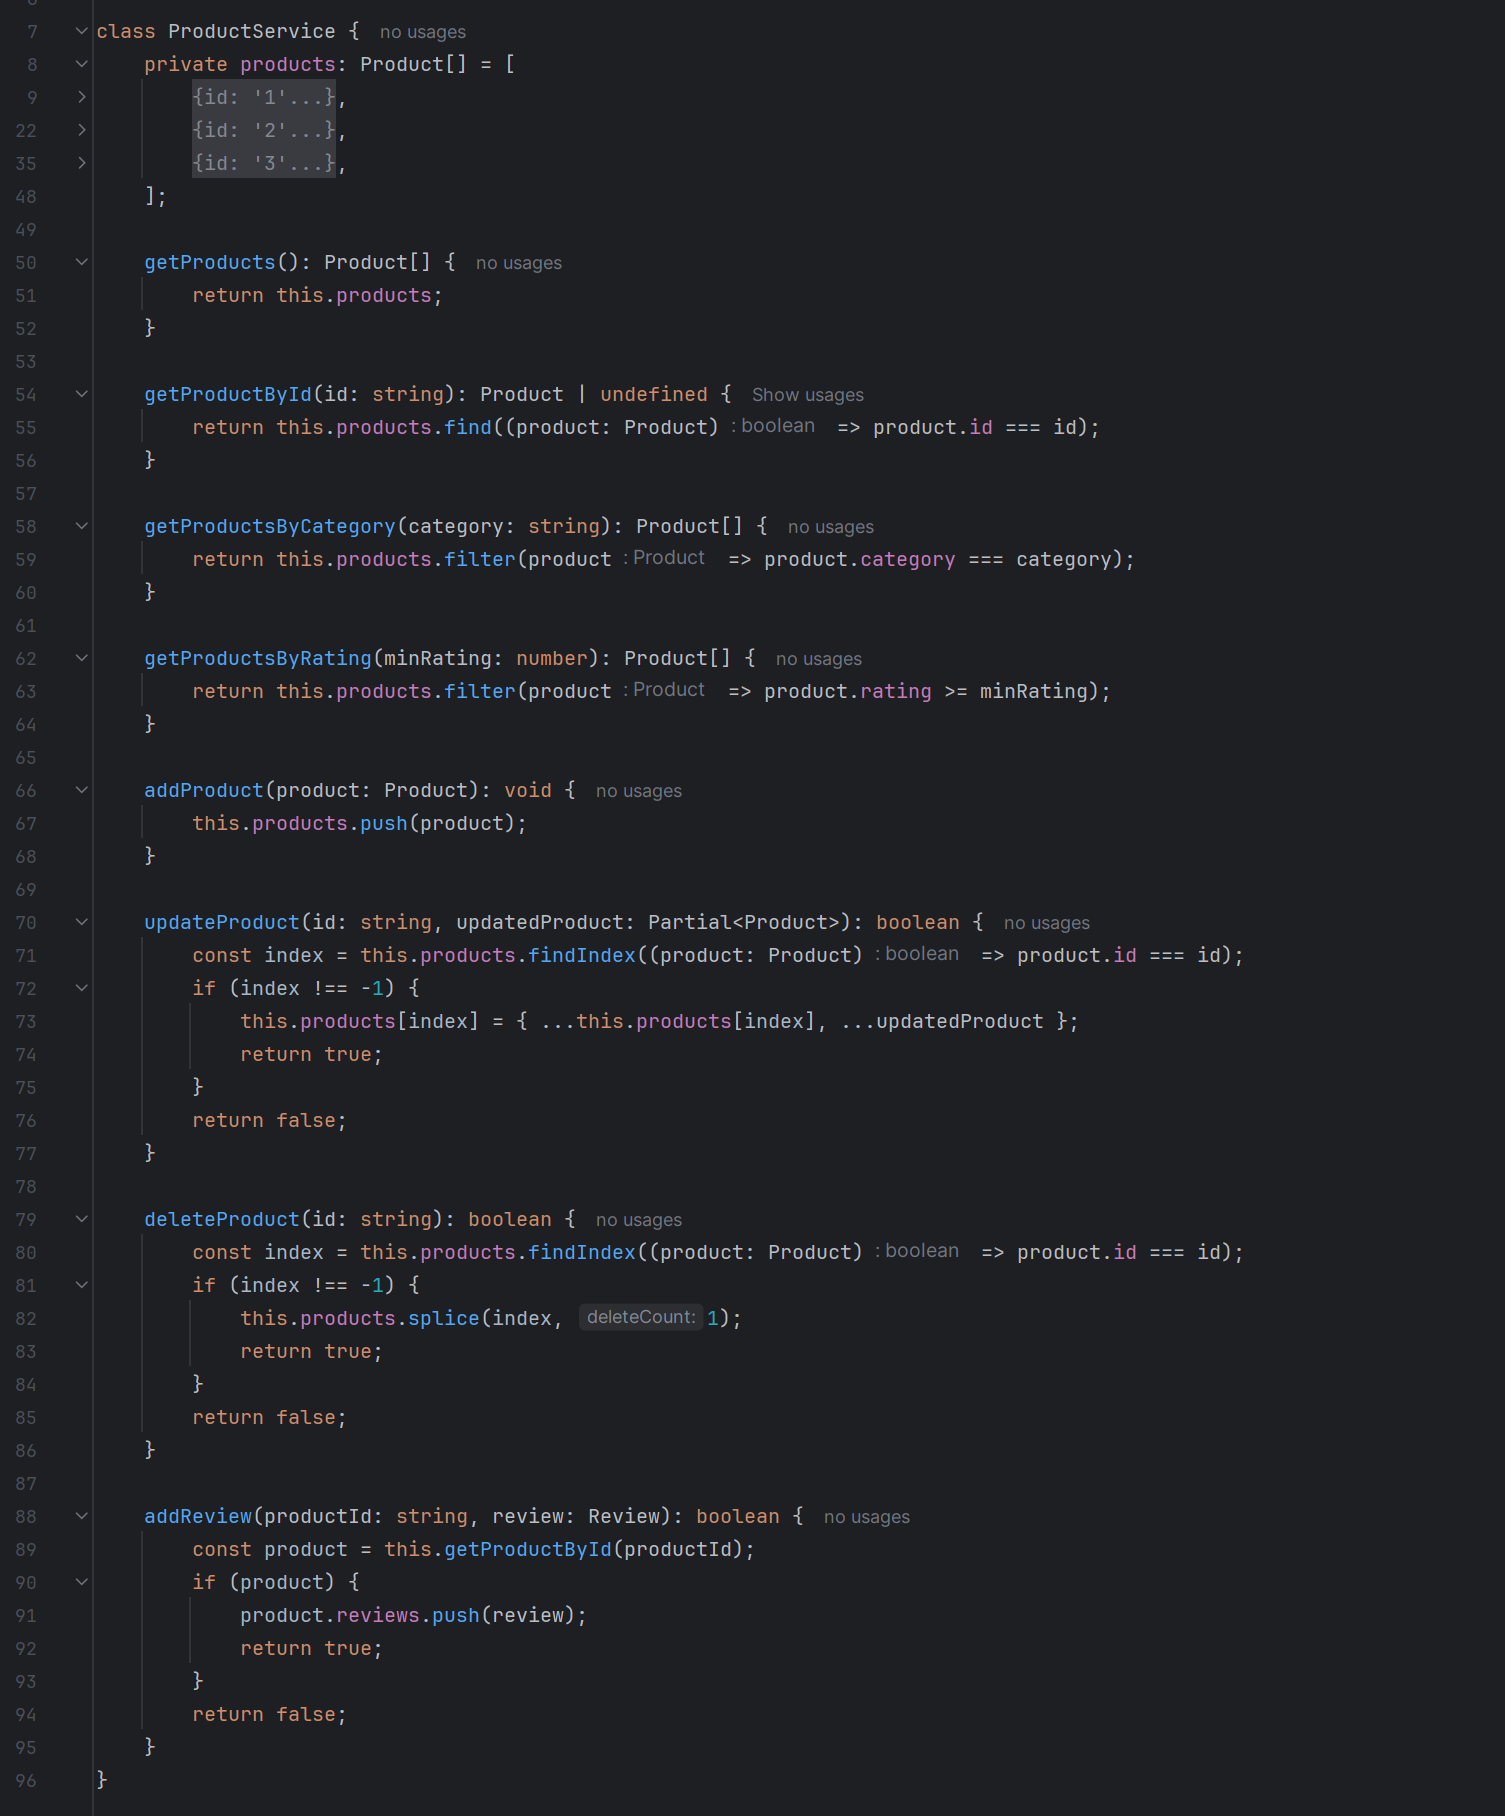
\includegraphics[width=0.7\paperwidth]{clean-code}}
            \end{center}
        }



        \section{Funkce}\label{sec:funkce}
        Samotné využívání funkcí představuje základní kámen v konstrukci čistého a efektivního kódu.
        Díky nim lze rozdělit program do logických bloků, což usnadňuje jeho strukturování a porozumění.
        Když je kód rozdělen do menších částí, je mnohem snazší sledovat jeho tok a identifikovat případné chyby nebo nedostatky.

        To znamená, že i složité úkoly mohou být rozloženy na menší, lépe řešitelné úseky, což v konečném důsledku vede k lepší údržbě a vývoji softwaru.
        Dalším klíčovým aspektem je znovupoužitelnost kódu díky funkcím.
        Pokud je správně navržena a implementována funkce, může být použita v různých částech programu nebo dokonce v jiných projektech.
        Tím se snižuje redundance kódu a zvyšuje se jeho modularita.
        Pokud je potřeba provést změnu, je často nutné upravit pouze jednu funkci, což minimalizuje riziko chyb a zjednodušuje úpravy.
        Tato schopnost znovu používat existující kód výrazně zlepšuje produktivitu vývojářů a zkracuje čas potřebný k vytvoření nových funkcí.

        Celkově lze tedy říci, že funkce nejsou pouze prostředkem k dosažení cíle, ale jsou základem pro efektivní a kvalitní vývoj softwarových projektů.
        Jejich správné využití přináší řadu výhod včetně zlepšené čitelnosti, snížení komplexity, lepší údržby a možnosti znovupoužití kódu, což v konečném důsledku vede k vyšší efektivitě a kvalitě výsledného produktu.

        \subsection{Výhody funkcí}\label{subsec:vyhody-funkci}
        \begin{itemize}
            \item Zlepšení čitelnosti: Funkce s dobrým názvem mohou sloužit jako komentáře, které vysvětlují, co určitá část kódu dělá.
            \item Usnadnění údržby: Úpravy v jedné funkci se obvykle nešíří do ostatních částí kódu, což snižuje riziko neočekávaných chyb.
            \item Zjednodušení testování: Jednotlivé funkce lze testovat izolovaně, což usnadňuje identifikaci chyb.
            \item Opakované využití kódu: Funkce umožňují znovupoužití kódu, což snižuje redundanci a usnadňuje změny.
        \end{itemize}

        \subsection{Nejlepší praktiky pro psaní funkcí}\label{subsec:nejlepsi-praktiky-pro-psani-funkci}
        \begin{itemize}
            \item Jedna funkce, jeden účel: Každá funkce by měla mít jedinou zodpovědnost, což usnadňuje její pochopení a údržbu.
            \item Krátké a jasné: Funkce by měly být co nejkratší, aniž by se obětovala čitelnost.
            Delší funkce je často možné rozdělit na menší, specializovanější funkce.
            \item Jasná pojmenování: Název funkce by měl jasně vysvětlovat, co funkce dělá.
            Vhodné pojmenování usnadňuje pochopení účelu funkce bez nutnosti prohlížet její implementaci.
            \item Omezení počtu parametrů: Funkce by měly mít co nejméně parametrů.
            Mnoho parametrů může funkci zkomplikovat a snížit její čitelnost.
            \item Používání návratových hodnot: Funkce by měly vracet hodnoty, které jasně indikují výsledek jejich provádění, což usnadňuje psaní čitelného a udržitelného kódu.
        \end{itemize}

        \subsection{Nevýhody a omezení}\label{subsec:nevyhody-a-omezeni}
        \begin{itemize}
            \item Nadužívání funkcí: Přílišné rozdělení kódu do funkcí může vést k nadbytečné abstrakci a zbytečné složitosti, což může ztížit pochopení toku programu.
            \item Výkonnostní kompromisy: V některých případech může volání funkcí způsobit mírné zpomalení, zejména v jazycích, kde je overhead volání funkcí významný.
            V kritických částech kódu, kde je výkon klíčový, je třeba zvážit rovnováhu mezi čistotou kódu a výkonem.
        \end{itemize}

        \break

        \subsection{Příklad funkce - Typescript}\label{subsec:priklad-funkce---typescript}
        Následující funkce v jazyce Typescript vrací \(n\)-tý prvek Fibonacciho posloupnosti:
        \begin{verbatim}
        function fibonacci(n: number): number {
            if (n <= 1) {
                return n;
            } else {
                return fibonacci(n - 1) + fibonacci(n - 2);
            }
        }
        \end{verbatim}

        \subsection{Příklad funkce - Python}\label{subsec:priklad-funkce---python}
        Následující funkce v jazyce Python vrací \(n\)-tý prvek Fibonacciho posloupnosti:
        \begin{verbatim}
        def fibonacci(n):
            if n <= 1:
                return n
            else:
                return fibonacci(n-1) + fibonacci(n-2)
        \end{verbatim}
    \end{Čistý kód - Funkce}

    \break

    \begin{Test Driven Development}
        \section{Test Driven Development}\label{sec:test-driven-development}

        Test Driven Development (TDD) je metodika vývoje softwaru, která klade důraz na testování.
        Testy jsou psány před samotným kódem a slouží jako specifikace požadované funkcionality.
        Tato metodika podporuje agilní vývoj a pomáhá vytvářet robustní a kvalitní software.

        \subsection{Historie a principy TDD}\label{subsec:historie-a-principy-tdd}

        TDD poprvé popsal Kent Beck v roce 1999 v knize \textbf{"Extreme Programming Explained"}.
        Metodika vychází z principů extrémního programování a zdůrazňuje následující:

        \begin{itemize}
            \item Testy před kódem: Než napíšete kód, nejprve napište test, který ověří požadovanou funkcionalitu.
            \item Malé kroky: Implementujte funkcionalitu v malých krocích, tak aby každý krok byl pokryt testy.
            \item Refaktoring: Po implementaci funkcionality proveďte refaktoring kódu, abyste jej zjednodušili a zlepšili jeho čitelnost.
        \end{itemize}

        \subsection{Výhody TDD}\label{subsec:vyhody-tdd}

        \begin{itemize}
            \item Zvýšená kvalita softwaru: TDD pomáhá odhalit chyby v rané fázi vývoje a snižuje tak počet chyb v produkčním kódu.
            \item Lepší design: TDD podporuje modularizaci kódu a jeho testování v izolaci, což vede k čistšímu a lépe strukturovanému designu.
            \item Větší jistota: TDD dává vývojářům jistotu, že kód funguje správně a splňuje požadavky.
            \item Lepší dokumentace: Testy slouží jako dokumentace požadované funkcionality.
        \end{itemize}

        \subsection{Nevýhody TDD}\label{subsec:nevyhody-tdd}

        \begin{itemize}
            \item Zvýšená náročnost: TDD vyžaduje disciplínu a zkušenost od vývojářů.
            \item Zvýšený čas: Psaní testů před kódem může zpočátku zdržet vývoj.
            \item Není vhodné pro všechny typy projektů: TDD nemusí být vhodné pro všechny typy projektů, například pro prototypování nebo rychlé dodávky.
        \end{itemize}

        \subsection{Implementace TDD}\label{subsec:implementace-tdd}

        Implementace TDD sestává z následujících kroků:

        \begin{enumerate}
            \item Definice požadavků: Jasně definujte požadavky na funkcionalitu, kterou chcete implementovat.
            \item Napsání testu: Napište test, který ověří požadovanou funkcionalitu.
            Test by měl být specifický, měřitelný, dosažitelný, relevantní a časově ohraničený.
            \item Implementace kódu: Implementujte kód, který splňuje požadavky testu.
            Začněte s nejjednodušší možnou implementací a postupně ji rozšiřujte.
            \item Refaktoring: Po implementaci kódu proveďte refaktoring, abyste jej zjednodušili a zlepšili jeho čitelnost.
            \item Opakování cyklu: Opakujte kroky 2 až 4 pro všechny požadované funkce.
        \end{enumerate}

        \subsection{Nástroje pro TDD}\label{subsec:nastroje-pro-tdd}

        Existuje mnoho nástrojů, které usnadňují implementaci TDD. Mezi nejoblíbenější patří:

        \begin{itemize}
            \item Testovací frameworky: Testovací frameworky, jako JUnit (Java) nebo NUnit (.NET), usnadňují psaní a spouštění testů.
            \item Mockingové frameworky: Mockingové frameworky, jako Mockito (Java) nebo Moq (.NET), umožňují simulovat závislosti v testech.
            \item Nástroje pro refaktoring: Nástroje pro refaktoring, jako IntelliJ IDEA (Java) nebo Visual Studio (.NET), usnadňují úpravu kódu bez narušení jeho funkcionality.
        \end{itemize}

        \break

        \subsection{Příklad - Typescript}\label{subsec:priklad---typescript}

        \textbf{\large Kód testující funkci validace emailu}
        \begin{verbatim}
            describe('validateEmail', () => {
              it('should return true for a valid email address', () => {
                expect(validateEmail('test@example.com')).toBe(true);
              });

              it('should return false for an invalid email address', () => {
                expect(validateEmail('test@example')).toBe(false);
                expect(validateEmail('testexample.com')).toBe(false);
                expect(validateEmail('@example.com')).toBe(false);
              });
            });
        \end{verbatim}

        \textbf{\large Funkce sloužící pro validaci emailu, psaná dle testu uvedeného výše}
        \begin{verbatim}
            export const validateEmail = (email: string): boolean => {
              const re = /^[^\s@]+@[^\s@]+\.[^\s@]+$/;
              return re.test(email);
            };
        \end{verbatim}

        \subsection{Shrnutí}\label{subsec:shrnuti}
        TDD je efektivní metodika vývoje softwaru, která pomáhá vytvářet robustní a kvalitní software.
        TDD vyžaduje disciplínu a zkušenost od vývojářů, ale přináší mnoho výhod, jako je zvýšená kvalita softwaru, lepší design a větší jistota.

    \end{Test Driven Development}

    \break

    \begin{Návrhový vzor - Command}
        \section{Návrhový vzor Command}
        Návrhový vzor Command zapouzdřuje operaci a její parametry do objektu, čímž umožňuje odložit provedení operace na později.
        To umožňuje flexibilnější a jednodušší implementaci logiky programu, jelikož umožňuje oddělit požadavek na provedení akce od jejího skutečného provedení.

        \subsection{Charakteristika}

        Návrhový vzor Command se skládá ze tří základních komponent:

        \begin{itemize}
            \item \textbf{Command (Příkaz)}: Definuje rozhraní pro provedení akce.
            Konkrétní implementace příkazu definuje, jaká akce se má provést.
            \item \textbf{Client (Klient)}: Vytváří instance příkazů a předává je objektu Invoker.
            \item \textbf{Invoker (Vyvolávač)}: Uchovává seznam příkazů a zodpovídá za jejich spuštění.
        \end{itemize}

        \subsection{Výhody}

        Návrhový vzor Command přináší mnoho výhod, mezi které patří:

        \begin{itemize}
            \item Zvýšená flexibilita: Umožňuje odložit provedení akce na později, čímž umožňuje dynamické plánování a spouštění akcí.
            \item Zjednodušení kódu: Odděluje logiku požadavku na provedení akce od logiky samotné akce, čímž umožňuje jednodušší a přehlednější kód.
            \item Podpora undo/redo funkcionality: Umožňuje snadno implementovat funkce pro vrácení a opakování provedených akcí, jelikož historii provedených akcí lze reprezentovat seznamem příkazů.
            \item Rozšířitelnost: Umožňuje snadno přidávat nové akce do systému, jelikož stačí implementovat novou třídu příkazu.
        \end{itemize}

        \subsection{Nevýhody}

        Návrhový vzor Command má i svá negativa, mezi která patří:

        \begin{itemize}
            \item Zvýšená režie: Zavedení objektu Command pro každou akci může vést k mírnému zvýšení režie.
            \item Složitější struktura: V porovnání s přímým voláním funkcí může struktura s objekty Command a Invoker působit složitěji.
        \end{itemize}

        \subsection{Příklad použití}

        Návrhový vzor Command se dá použít v široké škále aplikací.
        Níže je uveden příklad jeho použití v grafickém uživatelském rozhraní (GUI):

        \begin{itemize}
            \item Tlačítka v GUI můžou reprezentovat objekty Command.
            Kliknutím na tlačítko se instance Command předá objektu Invoker, který ji následně spustí.
            \item Makra v textových editorech můžou být implementována pomocí vzoru Command.
            Makro se skládá ze seznamu příkazů, které se po spuštění makra postupně provedou.
            \item Historie příkazů v grafických programech můžou být implementovány pomocí vzoru Command.
            Historie uchovává seznam provedených příkazů, které se dají zpětně spustit nebo vrátit zpět.
        \end{itemize}
    \end{Návrhový vzor - Command}
\end{document}
